\documentclass{article}
\usepackage[utf8]{inputenc}
\usepackage{graphicx}
\usepackage{epstopdf}
\usepackage{caption}
\usepackage{subcaption}
\usepackage{multirow}
\usepackage{hyperref}
\usepackage{url}
\usepackage{seqsplit}
\hypersetup{pdfstartview={FitH null null null}}
\usepackage{amssymb,amsmath}
\usepackage{amsthm}
\usepackage{empheq}
\usepackage{algorithm,algpseudocode}
\usepackage[margin=1.5in]{geometry}


\usepackage{listings}
\usepackage{color} %red, green, blue, yellow, cyan, magenta, black, white
\definecolor{mygreen}{RGB}{28,172,0} % color values Red, Green, Blue
\definecolor{mylilas}{RGB}{170,55,241}


\title{Template based modeling using a homology-based algorithm}
\author{Xiaokai Qian, Sean Lander, Caiwei Wang, Haipei Fan, Puneet Gaddam, Brett Koonce\\University of Missouri - Columbia}

\date{Feburary 18, 2013}

\algloopdefx{NoEndIf}[1]{\textbf{If} #1 \textbf{then}}

\begin{document}

\maketitle

\section{Abstract}
We implement basic homology (template) modeling of a DNA protein from CASP, T0644.  First, we search (BLAST) for templates that match our sequence.  Then, we align (BLOSUM62) our target sequence with the best template (3U1W).  Next, we build a copy of the the first protein's backbone using the template data wherever possible (our custom python tool).  Then, we fill in the gaps in our backbone using loop modeling (SCWRL) to produce a candidate PDB file.  Finally, we optimize (3D-Refine) our machine-generated PDB file.  Ultimately, we visualize (PyMOL) our results against the known structure of the protein and discuss how to improve our method.

\section{Introduction}

Template modeling is a technique very popular in bioinformatics.  First, we begin with a DNA sequence of unknown structure.  By searching a database of known sequences, we can find similar proteins to our unknown target.  Then we can build a model of our target by using known elements from other proteins.\\\\
When the two sequences do not differ greatly, this approach can generate usable models far quicker than traditional methods (real-world x-ray crystal modeling can take years to produce a single structure).  However, this approach is not foolproof.  Of considerable importance is filling in the gaps (loop modeling) in the differences between the two sequences, as well as making sure the final molecule is still a viable real-world model.\\\\
For our project, we implemented basic homology modeling in python, using a number of external tools to produce a pipeline capable of taking initial input sequence and presenting a final visualized model.



\subsection{Pipeline}
\begin{figure}[H]
\begin{center}
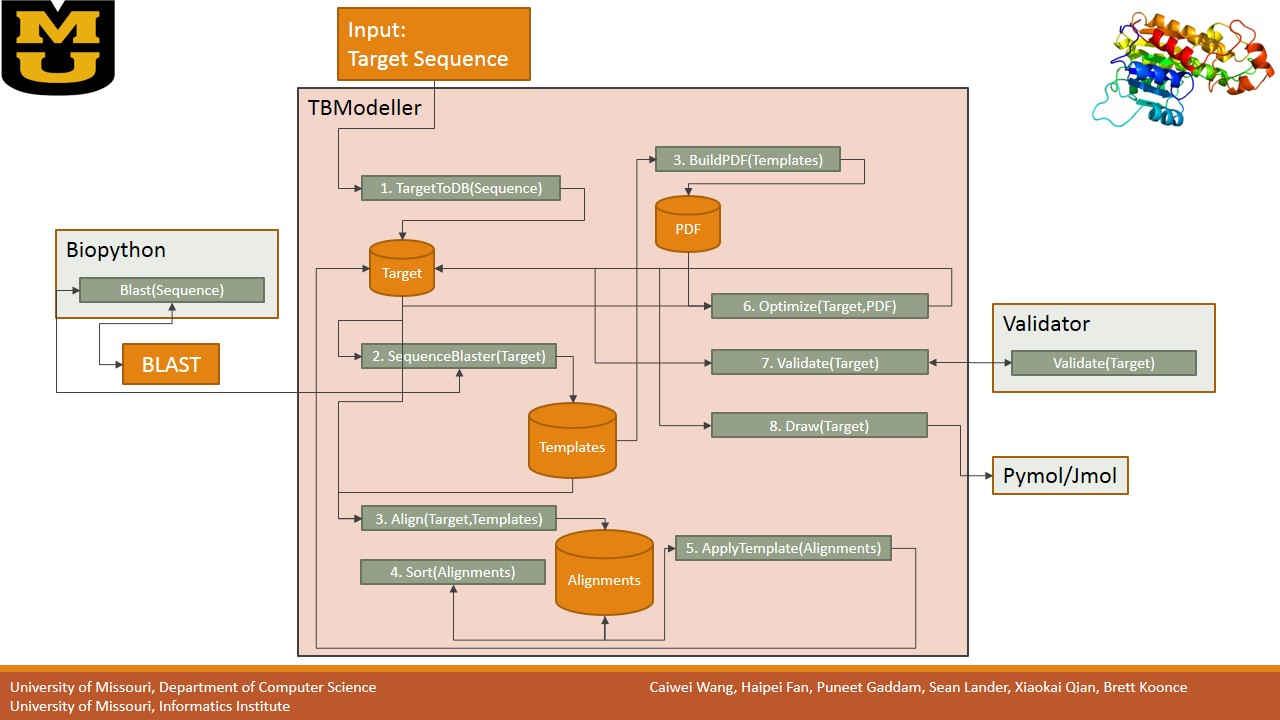
\includegraphics[width=\textwidth]{workflow}
\caption{An overview of the TBPy pipeline}
\label{Fig:blosum}
\end{center}
\end{figure}

\section{Algorithm}

\section{Template Search}

\section{Building a protein}

\section{Loop refinement and optimization}

\section{Visualization and results}

\end{document}


\end{document}
